\documentclass[12pt]{article}
\usepackage{amsfonts, amssymb, amsmath, amsthm}
\usepackage[margin=1in]{geometry}
\usepackage{tikz}
\usetikzlibrary{patterns, decorations.pathreplacing}

\pagestyle{myheadings}
\markright{Explainer: Rudin 4.4 --- Dense Images and Uniqueness\hfill}

\newcommand{\R}{\mathbb{R}}
\newcommand{\Q}{\mathbb{Q}}
\newcommand{\eps}{\varepsilon}

\begin{document}

\begin{center}
    \textbf{\Large Dense Images and Uniqueness of Continuous Maps}\\[0.5em]
    \large A visual guide to Rudin 4.4
\end{center}

\section{Quick Review: What Does ``Dense'' Mean?}

A subset $E \subseteq X$ is \textbf{dense} if $\overline{E} = X$: every point of $X$ is either in $E$ or a limit point of $E$.

Equivalently: every open ball in $X$ contains a point of $E$.

\begin{center}
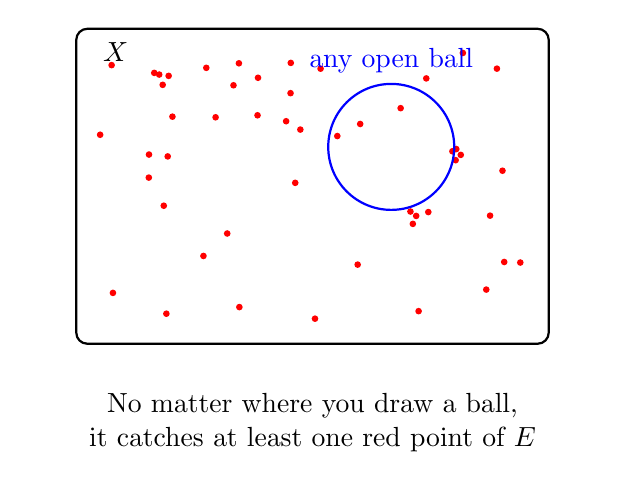
\begin{tikzpicture}[scale=1]
    % The space X
    \draw[thick, rounded corners] (-3, -2) rectangle (3, 2);
    \node at (-2.5, 1.7) {$X$};

    % Dense points
    \foreach \i in {1,...,50} {
        \pgfmathsetmacro{\x}{-2.7 + 5.4*rnd}
        \pgfmathsetmacro{\y}{-1.7 + 3.4*rnd}
        \fill[red] (\x, \y) circle (1.2pt);
    }

    % An open ball
    \draw[blue, thick] (1, 0.5) circle (0.8);
    \node[blue] at (1, 1.6) {any open ball};

    \node[text width=7cm, align=center] at (0, -3) {No matter where you draw a ball,\\it catches at least one red point of $E$};
\end{tikzpicture}
\end{center}

\section{Part 1: $f(E)$ is Dense in $f(X)$}

\textbf{Goal:} If $f: X \to Y$ is continuous and $E$ is dense in $X$, then $f(E)$ is dense in $f(X)$.

\textbf{What this means:} Every point in the image $f(X)$ can be approximated by points in $f(E)$.

\begin{center}
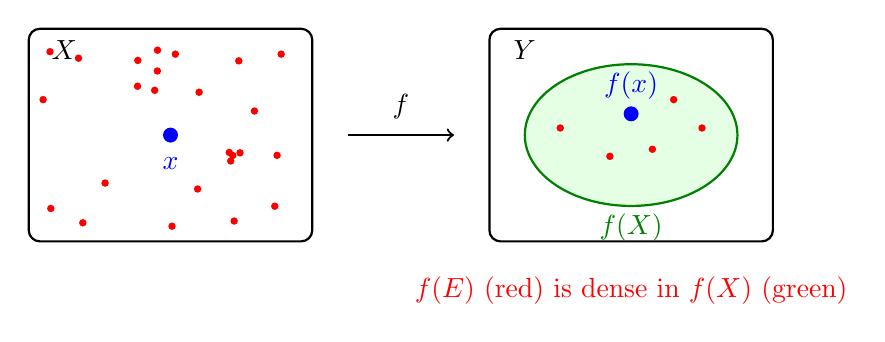
\begin{tikzpicture}[scale=0.9]
    % Domain X
    \draw[thick, rounded corners] (-5, -1.5) rectangle (-1, 1.5);
    \node at (-4.5, 1.2) {$X$};

    % Dense points in X
    \foreach \i in {1,...,25} {
        \pgfmathsetmacro{\x}{-4.8 + 3.6*rnd}
        \pgfmathsetmacro{\y}{-1.3 + 2.6*rnd}
        \fill[red] (\x, \y) circle (1.5pt);
    }

    % A point x in X
    \fill[blue] (-3, 0) circle (3pt);
    \node[blue] at (-3, -0.4) {$x$};

    % Arrow for f
    \draw[->, thick] (-0.5, 0) -- (1, 0);
    \node at (0.25, 0.4) {$f$};

    % Codomain Y
    \draw[thick, rounded corners] (1.5, -1.5) rectangle (5.5, 1.5);
    \node at (2, 1.2) {$Y$};

    % Image f(X) inside Y
    \draw[green!50!black, thick, fill=green!10] (3.5, 0) ellipse (1.5 and 1);
    \node[green!50!black] at (3.5, -1.3) {$f(X)$};

    % f(x)
    \fill[blue] (3.5, 0.3) circle (3pt);
    \node[blue] at (3.5, 0.7) {$f(x)$};

    % f(E) points
    \fill[red] (2.5, 0.1) circle (1.5pt);
    \fill[red] (3.2, -0.3) circle (1.5pt);
    \fill[red] (4.1, 0.5) circle (1.5pt);
    \fill[red] (3.8, -0.2) circle (1.5pt);
    \fill[red] (4.5, 0.1) circle (1.5pt);

    \node[red] at (3.5, -2.2) {$f(E)$ (red) is dense in $f(X)$ (green)};
\end{tikzpicture}
\end{center}

\subsection{The Key Idea}

\begin{center}
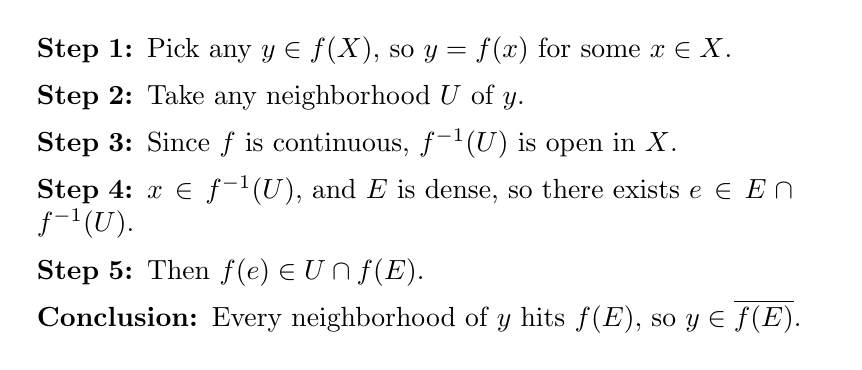
\begin{tikzpicture}[scale=1]
    \node[text width=10cm, align=left] at (0, 0) {
        \textbf{Step 1:} Pick any $y \in f(X)$, so $y = f(x)$ for some $x \in X$.\\[0.5em]
        \textbf{Step 2:} Take any neighborhood $U$ of $y$.\\[0.5em]
        \textbf{Step 3:} Since $f$ is continuous, $f^{-1}(U)$ is open in $X$.\\[0.5em]
        \textbf{Step 4:} $x \in f^{-1}(U)$, and $E$ is dense, so there exists $e \in E \cap f^{-1}(U)$.\\[0.5em]
        \textbf{Step 5:} Then $f(e) \in U \cap f(E)$.\\[0.5em]
        \textbf{Conclusion:} Every neighborhood of $y$ hits $f(E)$, so $y \in \overline{f(E)}$.
    };
\end{tikzpicture}
\end{center}

\begin{center}
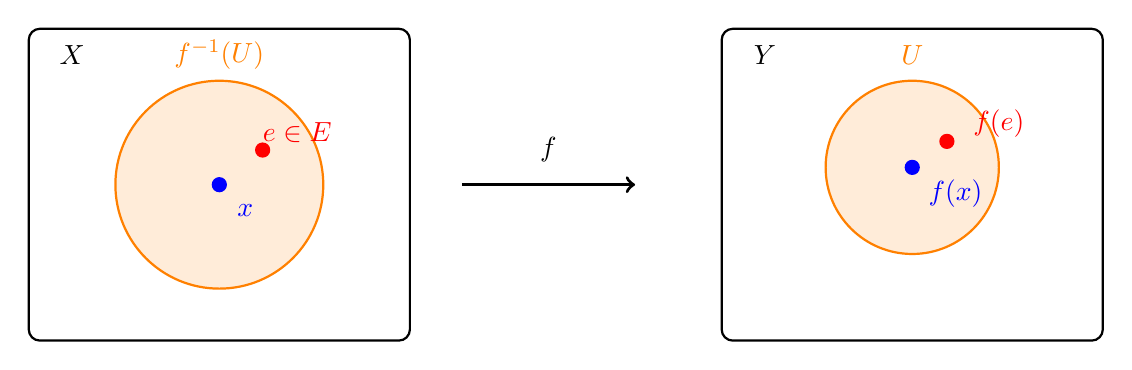
\begin{tikzpicture}[scale=1.1]
    % X side
    \begin{scope}[xshift=-4cm]
        \draw[thick, rounded corners] (-2.2, -1.8) rectangle (2.2, 1.8);
        \node at (-1.7, 1.5) {$X$};

        % f^{-1}(U)
        \draw[orange, thick, fill=orange!15] (0, 0) circle (1.2);
        \node[orange] at (0, 1.5) {$f^{-1}(U)$};

        % x
        \fill[blue] (0, 0) circle (2.5pt);
        \node[blue] at (0.3, -0.3) {$x$};

        % e in E
        \fill[red] (0.5, 0.4) circle (2.5pt);
        \node[red] at (0.9, 0.6) {$e \in E$};
    \end{scope}

    % Arrow
    \draw[->, very thick] (-1.2, 0) -- (0.8, 0);
    \node at (-0.2, 0.4) {$f$};

    % Y side
    \begin{scope}[xshift=4cm]
        \draw[thick, rounded corners] (-2.2, -1.8) rectangle (2.2, 1.8);
        \node at (-1.7, 1.5) {$Y$};

        % U
        \draw[orange, thick, fill=orange!15] (0, 0.2) circle (1);
        \node[orange] at (0, 1.5) {$U$};

        % f(x)
        \fill[blue] (0, 0.2) circle (2.5pt);
        \node[blue] at (0.5, -0.1) {$f(x)$};

        % f(e)
        \fill[red] (0.4, 0.5) circle (2.5pt);
        \node[red] at (1, 0.7) {$f(e)$};
    \end{scope}
\end{tikzpicture}
\end{center}

\section{Part 2: Continuous Maps Agree Everywhere if They Agree on a Dense Set}

\textbf{Goal:} If $f(p) = g(p)$ for all $p \in E$ (dense), then $f = g$ on all of $X$.

\begin{center}
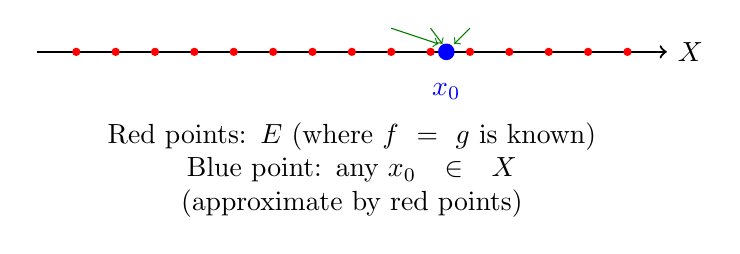
\begin{tikzpicture}[scale=1]
    % Number line representing X
    \draw[thick, ->] (-4, 0) -- (4, 0);
    \node at (4.3, 0) {$X$};

    % Dense points where f = g
    \foreach \x in {-3.5, -3, -2.5, -2, -1.5, -1, -0.5, 0, 0.5, 1, 1.5, 2, 2.5, 3, 3.5} {
        \fill[red] (\x, 0) circle (1.5pt);
    }

    % A point x0 not in E
    \fill[blue] (1.2, 0) circle (3pt);
    \node[blue] at (1.2, -0.5) {$x_0$};

    % Arrows showing approximation
    \draw[green!50!black, ->] (0.5, 0.3) -- (1.1, 0.1);
    \draw[green!50!black, ->] (1.5, 0.3) -- (1.3, 0.1);
    \draw[green!50!black, ->] (1, 0.3) -- (1.15, 0.1);

    \node[text width=8cm, align=center] at (0, -1.5) {Red points: $E$ (where $f = g$ is known)\\Blue point: any $x_0 \in X$ (approximate by red points)};
\end{tikzpicture}
\end{center}

\subsection{Why Must $f(x_0) = g(x_0)$?}

\begin{center}
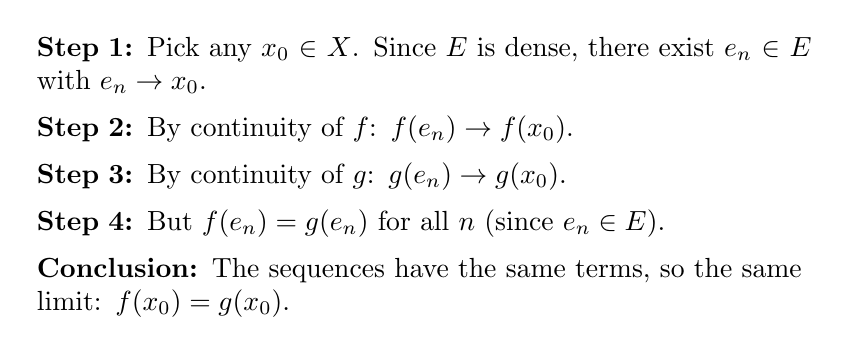
\begin{tikzpicture}[scale=1]
    \node[text width=10cm, align=left] at (0, 0) {
        \textbf{Step 1:} Pick any $x_0 \in X$. Since $E$ is dense, there exist $e_n \in E$ with $e_n \to x_0$.\\[0.5em]
        \textbf{Step 2:} By continuity of $f$: $f(e_n) \to f(x_0)$.\\[0.5em]
        \textbf{Step 3:} By continuity of $g$: $g(e_n) \to g(x_0)$.\\[0.5em]
        \textbf{Step 4:} But $f(e_n) = g(e_n)$ for all $n$ (since $e_n \in E$).\\[0.5em]
        \textbf{Conclusion:} The sequences have the same terms, so the same limit: $f(x_0) = g(x_0)$.
    };
\end{tikzpicture}
\end{center}

\begin{center}
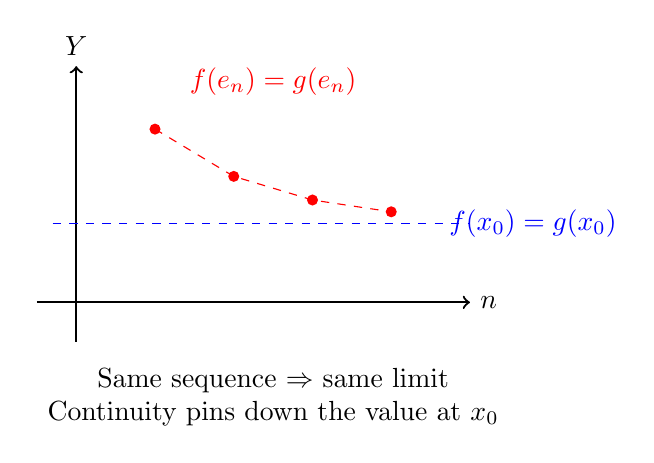
\begin{tikzpicture}[scale=1]
    % Two function graphs converging
    \draw[thick, ->] (-0.5, 0) -- (5, 0) node[right] {$n$};
    \draw[thick, ->] (0, -0.5) -- (0, 3) node[above] {$Y$};

    % f(e_n) = g(e_n) values converging
    \fill[red] (1, 2.2) circle (2pt);
    \fill[red] (2, 1.6) circle (2pt);
    \fill[red] (3, 1.3) circle (2pt);
    \fill[red] (4, 1.15) circle (2pt);

    \draw[red, dashed] (1, 2.2) -- (2, 1.6) -- (3, 1.3) -- (4, 1.15);

    % Limit
    \draw[blue, dashed] (-0.3, 1) -- (5, 1);
    \node[blue] at (5.8, 1) {$f(x_0) = g(x_0)$};

    \node[red] at (2.5, 2.8) {$f(e_n) = g(e_n)$};

    \node[text width=6cm, align=center] at (2.5, -1.2) {Same sequence $\Rightarrow$ same limit\\Continuity pins down the value at $x_0$};
\end{tikzpicture}
\end{center}

\section{The Big Picture}

\begin{center}
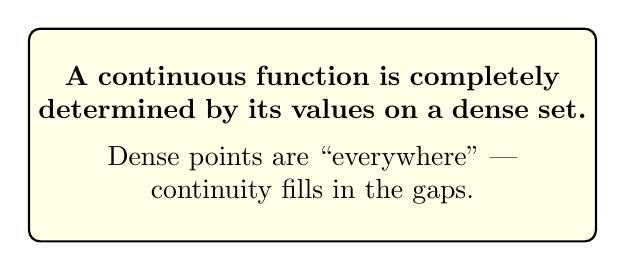
\begin{tikzpicture}[scale=0.9]
    \draw[thick, rounded corners, fill=yellow!10] (-4, -1.5) rectangle (4, 1.5);

    \node[text width=7cm, align=center] at (0, 0) {
        \textbf{A continuous function is completely}\\
        \textbf{determined by its values on a dense set.}\\[0.5em]
        Dense points are ``everywhere'' ---\\
        continuity fills in the gaps.
    };
\end{tikzpicture}
\end{center}

\textbf{Analogy:} If you know the temperature at every rational time, and temperature varies continuously, you know it at every real time too. The rationals are dense in $\R$, so there are no ``gaps'' that continuity can't bridge.

\end{document}
